\section{Deep learning}

\newcommand{\polynomialplot}[1]{
    \begin{tikzpicture}
        \begin{axis}[
            height=6cm,
            width=6cm,
            xmin=-1.6,
            xmax=1.6,
            ymin=0,
            ymax=5,
            xmajorticks=false,
            ymajorticks=false,
            xlabel=$x$,
            ylabel=$y$
        ]
            \addplot[
                samples=100,
                domain=-1.6:1.6,
                only marks,
                blue,
                opacity=0.5
            ] (x, {x^4-3*x^2-x+4+0.5*rand});

            \ifnum#1=1
                \addplot[
                    samples=100,
                    domain=-1.6:1.6,
                    red,
                    very thick
                ] (x, {x^4-3*x^2-x+4});
            \fi
            \ifnum#1=2
                \addplot[
                    samples=100,
                    domain=-1.6:1.6,
                    red,
                    very thick
                ] coordinates {
                    (-1.6, 4.4)
                    (-1.4, 4.4)
                    (-1.4, 3)
                    (-0.8, 3)
                    (-0.8, 4)
                    (0.2, 4)
                    (0.2, 3)
                    (0.6, 3)
                    (0.6, 2)
                    (0.8, 2)
                    (0.8, 0.8)
                    (1.6, 0.8)
                };
            \fi
            \ifnum#1=3
                \addplot[
                    samples=100,
                    domain=-1.6:1.6,
                    red,
                    very thick
                ] (x, {x^4-3*x^2-x+4+0.1*rand});
            \fi
            \ifnum#1=4
                \addplot[
                    samples=100,
                    domain=-1.6:1.6,
                    red,
                    very thick
                ] coordinates {
                    (-1.6, 4.4)
                    (-1.4, 3)
                    (-1.3, 2.9)
                    (-1.1, 2.9)
                    (-0.5, 3.8)
                    (0, 3.8)
                    (0.4, 3)
                    (1, 1)
                    (1.2, 0.7)
                    (1.6, 1.2)
                };
            \fi
        \end{axis}
    \end{tikzpicture}
}

\newsavebox{\polynomialdata}
\sbox{\polynomialdata}{
    \polynomialplot{0}
}
\newsavebox{\polynomialspline}
\sbox{\polynomialspline}{
    \polynomialplot{1}
}
\newsavebox{\polynomialtree}
\sbox{\polynomialtree}{
    \polynomialplot{2}
}
\newsavebox{\polynomialpiecewise}
\sbox{\polynomialpiecewise}{
    \polynomialplot{3}
}
\newsavebox{\polynomialapprox}
\sbox{\polynomialapprox}{
    \polynomialplot{4}
}

\newsavebox{\correlatedpredictors}
\sbox{\correlatedpredictors}{
    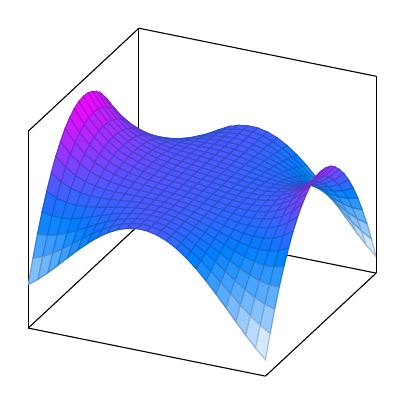
\begin{tikzpicture}
        \begin{axis}[
            height=6cm,
            width=6cm,
            xmajorticks=false,
            ymajorticks=false,
            zmajorticks=false
        ]
            \addplot3 [
                surf,
                domain=-1.5:1.5,
                y domain=-1.5:1.5,
                colormap/cool,
                draw=black
            ] {{x^4-3*(x*y)^2-x+4}};
        \end{axis}
    \end{tikzpicture}
}
\begin{frame}{Deep learning: Motivation}
    \begin{tikzpicture}
        \node[draw=black] at (-5.25, 3.5) {};
        \node[draw=black] at (5.25, -3.5) {};

        \visible<1,6>{
            \node[] at (0, 0.5) {
                \usebox{\polynomialdata}
            };
        }
        %shader=interp,
        \visible<2>{
            \node[] at (0, 0.5) {
                \usebox{\polynomialspline}
            };
            \node[font=\small] at (0, -2.75) {
                $\hat{y}=s(x)$
            };
        }
        \visible<3>{
            \node[] at (0, 0.5) {
                \usebox{\polynomialtree}
            };
            \node[font=\small] at (0, -2.75) {
                $\hat{y}=
                \begin{cases}
                    4&\cdots\\
                    3&0.2\leq x<0.6\\
                    1.5&\cdots\\
                \end{cases}
                $
            };
        }
        \visible<4>{
            \node[] at (0, 0.5) {
                \usebox{\correlatedpredictors}
            };
        }
        \visible<5>{
            \node[inner sep=0pt, draw=black] at (-2.5, 0) {
                \includegraphics[width=3cm]{data/cat.png}
            };
            \node[align=center, draw=black] at (2.5, 0) {
                The cat wagged\\ its tail
            };
        }
        \visible<7>{
            \node[] at (0, 0.5) {
                \usebox{\polynomialpiecewise}
            };
        }
    \end{tikzpicture}
\end{frame}

\newsavebox{\threedimensional}
\sbox{\threedimensional}{
    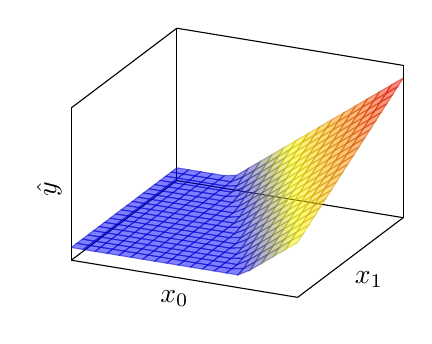
\begin{tikzpicture}[
        declare function = {
            q(\x) = \x - 1;
            Z(\x,\y) = max(0, \x*0.5 + \y*0.25);
        }
    ]
        \begin{axis}
        [
            height=5cm,
            ticks=none,
            xlabel=$x_0$,
            ylabel=$x_1$,
            zlabel=$\hat{y}$,
            domain=-1:1,
            samples=20,
        ]
            \addplot3 [surf, opacity=0.5] {Z(x,y)};
        \end{axis}
    \end{tikzpicture}
}

\begin{frame}{Deep learning: Artificial neural networks}

    \def\nodesize{14pt}
    \colorlet{nodefill}{teal!40}

    \newcommand{\artificialneuron}[3]{
        \node[
            circle,
            draw=black,
            fill=nodefill,
            minimum size=\nodesize,
            inner sep=0pt
        ] (####2) at ####1 {};

        % \ifnum####1=1

        % \fi
    }

    \centering
    \begin{tikzpicture}
        \node[] at (-5, 3) {};
        \node[] at (5, -4.5) {};

        \visible<1>{
            \artificialneuron{(0, 1.5)}{n}{0}
            \node[] (x) at (-1.5, 1.5) {$x$};
            \node[] (b) at (0, 2.5) {$\beta_0$};
            \node[] (y) at (1.5, 1.5) {$\hat{y}$};

            \draw[->] (x) -- (n) node [midway, above] {$\beta_1$};
            \draw[->] (b) -- (n);
            \draw[->] (n) -- (y);

            \node[] at (0, 0) {$\hat{y}=\beta_0+\beta_1x$};
        }

        \visible<2-3>{
            \node[] at (0, 0) {$\hat{y}=wx+b$};
        }
        \visible<2-5>{
            \artificialneuron{(0, 1.5)}{n}{0}
            \node[] (x) at (-1.5, 1.5) {$x$};
            \node[] (b) at (0, 2.5) {$b$};
            \node[] (y) at (1.5, 1.5) {$\hat{y}$};

            \draw[->] (x) -- (n) node [midway, above] {$w$};
            \draw[->] (b) -- (n);
            \draw[->] (n) -- (y);
        }
        \visible<3>{
            \draw[] (-2, -1.5) -- (2, -1.5) -- (2, -4) -- (-2, -4) -- (-2, -1.5);

            \draw[very thick, blue!60] (-2, -3.5) -- (2, -1.75);

            \node[anchor=north] at (0, -4.1) {x};
            \node[anchor=south, rotate=90] at (-2.1, -2.75) {$\hat{y}$};
        }
        \visible<4>{
            \node[] at (0, 0) {$\hat{y}=\dfrac{e^x}{1+e^x}$};

            \node[anchor=south, font=\footnotesize\selectfont] at (0, -1.5) {Sigmoid};

            \draw[] (-2, -1.5) -- (2, -1.5) -- (2, -4) -- (-2, -4) -- (-2, -1.5);
            \draw[very thick, blue!60, smooth] (-2, -3.5) -- (-1, -3.5) to[in=180, out=0] (1, -1.75) -- (2, -1.75);

            \node[anchor=north] at (0, -4.1) {x};
            \node[anchor=south, rotate=90] at (-2.1, -2.75) {$\hat{y}$};
        }
        \visible<5>{
            \node[] at (0, 0) {$\hat{y}=max(0, wx+b)$};

            \node[anchor=south, font=\footnotesize\selectfont] at (0, -1.5) {Rectified Linear Unit (ReLU)};

            \draw[] (-2, -1.5) -- (2, -1.5) -- (2, -4) -- (-2, -4) -- (-2, -1.5);
            \draw[very thick, blue!60] (-2, -3.5) -- (0, -3.5) -- (2, -1.75);

            \node[anchor=north] at (0, -4.1) {x};
            \node[anchor=south, rotate=90] at (-2.1, -2.75) {$\hat{y}$};
        }
        \visible<6>{
            \artificialneuron{(0, 2)}{n0}{0}
            \artificialneuron{(0, 1)}{n1}{0}

            \node[] (x) at (-1.5, 1.5) {$x$};
            \node[] (y) at (1.5, 1.5) {$\hat{y}$};
            \node[] at (0, 0) {$\hat{y}=max(0, w_0x+b_0)+max(0, w_1x+b_1)$};

            \draw[->] (x) -- (n0) node [midway, above] {$w_0$};
            \draw[->] (x) -- (n1) node [midway, below] {$w_1$};
            \draw[->] (n0) -- (y);
            \draw[->] (n1) -- (y);

            \draw[] (-2, -1.5) -- (2, -1.5) -- (2, -4) -- (-2, -4) -- (-2, -1.5);
            \draw[very thick, blue!60] (-2, -3.5) -- (-0.66, -3.5) -- (0.66, -2.25) -- (2, -3);

            \node[anchor=north] at (0, -4.1) {x};
            \node[anchor=south, rotate=90] at (-2.1, -2.75) {$\hat{y}$};
        }
        \visible<7>{
            \node[] at (0, 0) {
                \usebox{\polynomialapprox}
            };
            \node[] at (0, -2.5) {
                Piecewise linear function
            };
        }
        \visible<8>{
            \node[align=center, text width=10cm] at (0, -0.75) {
                \textbf{Universal approximation theorem:}\\
                \begin{quotation}
                    \centering
                    "Any relationship that can be described with a polynomial function can be approximated by a neural network with a single hidden layer."
                \end{quotation}
            };
        }
        \visible<9>{
            \artificialneuron{(0, 1.5)}{n}{0}

            \node[] (x0) at (-1.5, 2) {$x_0$};
            \node[] (x1) at (-1.5, 1) {$x_1$};
            \node[] (b) at (0, 2.5) {$b$};
            \node[] (y) at (1.5, 1.5) {$\hat{y}$};
            \node[] at (0, 0) {$\hat{y}=max(0, w_0x_0+w_1x_1+b)$};

            \draw[->] (x0) -- (n) node [midway, above] {$w_0$};
            \draw[->] (x1) -- (n) node [midway, below] {$w_1$};
            \draw[->] (b) -- (n);
            \draw[->] (n) -- (y);

            \node[] at (0, -2.75) {
                \usebox{\threedimensional}
            };
        }
        \visible<10-13>{
            \artificialneuron{(0, 2)}{n00}{0}
            \artificialneuron{(0, 1)}{n01}{0}
        }
        \visible<10>{
            \node[
                circle,
                minimum size=\nodesize,
                inner sep=0pt,
                text depth=0
            ] (x) at (-3, 1.5) {\footnotesize{$x$}};

            \node[
                circle,
                minimum size=\nodesize,
                inner sep=0pt,
                text depth=0
            ] (y) at (3, 1.5) {\footnotesize{$\hat{y}$}};

            \draw[->] (x) -- (n00) node [midway, above] {$w_0$};
            \draw[->] (x) -- (n01) node [midway, below] {$w_1$};

            \draw[->] (n00) -- (y);
            \draw[->] (n01) -- (y);

            \def\spacing{-0.1cm}
            \node[anchor=north] at (0, 0) {\tiny{
                \begin{math}
                    \begin{alignedat}{5}
                        \hat{y} = max(0, w_0x+b_0)+max(0, w_1x+b_1)\\
                    \end{alignedat}
                \end{math}
            }};
        }
        \visible<11-12>{
            \node[
                circle,
                draw=black,
                fill=nodefill,
                minimum size=\nodesize,
                inner sep=0pt,
                text depth=0
            ] (x) at (-3, 1.5) {\footnotesize{$x$}};

            \draw[->] (x) -- (n00) node [midway, above] {$w^0_0$};
            \draw[->] (x) -- (n01) node [midway, below] {$w^0_1$};

            \def\spacing{-0.1cm}
            \node[anchor=north] at (0, 0) {\tiny{
                \begin{math}
                    \begin{alignedat}{5}
                        \hat{y} = max(0, w^1_0*max(0, w^0_0*x+b^0_0)+w^1_1*max(0, w^0_1*x+b^0_1)+b^1_0)\\
                    \end{alignedat}
                \end{math}
            }};
        }
        \visible<11-15>{
            \node[
                circle,
                draw=black,
                fill=nodefill,
                minimum size=\nodesize,
                inner sep=0pt,
                text depth=0
            ] (y) at (3, 1.5) {\footnotesize{$\hat{y}$}};
        }
        \visible<11-12>{
            \draw[->] (n00) -- (y) node [midway, above] {$w^1_0$};
            \draw[->] (n01) -- (y) node [midway, below] {$w^1_1$};
        }
        \visible<12>{
            \node[text depth=0] at (-3, 0.3) {\textcolor{red}{Input}};
            \node[text depth=0] at (0, 0.3) {\textcolor{red}{Hidden}};
            \node[text depth=0] at (3, 0.3) {\textcolor{red}{Output}};
        }
        \visible<13-15>{
            \node[
                circle,
                draw=black,
                fill=nodefill,
                minimum size=\nodesize,
                inner sep=0pt,
                text depth=0
            ] (x0) at (-3, 2) {\footnotesize{$x_0$}};
            \node[
                circle,
                draw=black,
                fill=nodefill,
                minimum size=\nodesize,
                inner sep=0pt,
                text depth=0
            ] (x1) at (-3, 1) {\footnotesize{$x_1$}};
        }
        \visible<13>{
            \draw[->] (x0) -- (n00);
            \draw[->] (x0) -- (n01);
            \draw[->] (x1) -- (n00);
            \draw[->] (x1) -- (n01);

            \node[anchor=north] at (0, 0) {\tiny{
                \begin{math}
                    \begin{alignedat}{5}
                        \hat{y} &= max(0, &&w^1_{0,0}*max(0, w^0_{0,0}*x_0+w^0_{1,0}*x_{1}+b_{0,0})+\\[\spacing]
                        & &&w^1_{1,0}*max(0, w^0_{0,1}*x_0+w^0_{1,1}*x_{1}+b_{0,1})+\\[\spacing]
                        & &&b_1)&&\\
                    \end{alignedat}
                \end{math}
            }};
        }
        \visible<14>{
            \artificialneuron{(0, 2.5)}{n00}{0}
            \artificialneuron{(0, 1.5)}{n01}{0}
            \artificialneuron{(0, 0.5)}{n02}{0}

            \draw[->] (x0) -- (n00);
            \draw[->] (x0) -- (n01);
            \draw[->] (x0) -- (n02);
            \draw[->] (x1) -- (n00);
            \draw[->] (x1) -- (n01);
            \draw[->] (x1) -- (n02);

            \draw[->] (n00) -- (y);
            \draw[->] (n01) -- (y);
            \draw[->] (n02) -- (y);

            \node[anchor=north] at (0, 0) {\tiny{
                \begin{math}
                    \begin{alignedat}{5}
                        \hat{y} &= max(0, &&w^1_{0,0}*max(0, w^0_{0,0}*x_0+w^0_{1,0}*x_{1}+b_{0,0})+\\[\spacing]
                        & &&w^1_{1,0}*max(0, w^0_{0,1}*x_0+w^0_{1,1}*x_{1}+b_{0,1})+\\[\spacing]
                        & &&w^1_{2,0}*max(0, w^0_{0,2}*x_0+w^0_{1,2}*x_{1}+b_{0,2})+\\[\spacing]
                        & &&b_1)&&\\
                    \end{alignedat}
                \end{math}
            }};
        }
        \visible<15>{
            \artificialneuron{(-1, 2.5)}{n00}{0}
            \artificialneuron{(-1, 1.5)}{n01}{0}
            \artificialneuron{(-1, 0.5)}{n02}{0}

            \artificialneuron{(1, 2.5)}{n10}{0}
            \artificialneuron{(1, 1.5)}{n11}{0}
            \artificialneuron{(1, 0.5)}{n12}{0}

            \draw[->] (x0) -- (n00);
            \draw[->] (x0) -- (n01);
            \draw[->] (x0) -- (n02);
            \draw[->] (x1) -- (n00);
            \draw[->] (x1) -- (n01);
            \draw[->] (x1) -- (n02);

            \draw[->] (n00) -- (n10);
            \draw[->] (n00) -- (n11);
            \draw[->] (n00) -- (n12);
            \draw[->] (n01) -- (n10);
            \draw[->] (n01) -- (n11);
            \draw[->] (n01) -- (n12);
            \draw[->] (n02) -- (n10);
            \draw[->] (n02) -- (n11);
            \draw[->] (n02) -- (n12);

            \draw[->] (n10) -- (y);
            \draw[->] (n11) -- (y);
            \draw[->] (n12) -- (y);

            \node[anchor=north] at (0, 0) {\tiny{
                \begin{math}
                    \begin{alignedat}{5}
                        \hat{y} &= max(0, &&w^2_{0,0}*max(0, &&w^1_{0,0}*max(0, w^0_{0,0}*x_0+w^0_{1,0}*x_{1}+b_{0,0})+\\[\spacing]
                        & && &&w^1_{1,0}*max(0, w^0_{0,1}*x_0+w^0_{1,1}*x_{1}+b_{0,1})+\\[\spacing]
                        & && &&w^1_{2,0}*max(0, w^0_{0,2}*x_0+w^0_{1,2}*x_{1}+b_{0,2})+\\[\spacing]
                        & && &&b_{1,0})+\\[\spacing]
                        & &&w^2_{1,0}*max(0, &&w^1_{0,1}*max(0, w^0_{0,0}*x_0+w^0_{1,0}*x_{1}+b_{0,0})+\\[\spacing]
                        & && &&w^1_{1,1}*max(0, w^0_{0,1}*x_0+w^0_{1,1}*x_{1}+b_{0,1})+\\[\spacing]
                        & && &&w^1_{2,1}*max(0, w^0_{0,2}*x_0+w^0_{1,2}*x_{1}+b_{0,2})+\\[\spacing]
                        & && &&b_{1,1})+\\[\spacing]
                        & &&w^2_{2,0}*max(0, &&w^1_{0,2}*max(0, w^0_{0,0}*x_0+w^0_{1,0}*x_{1}+b_{0,0})+\\[\spacing]
                        & && &&w^1_{1,2}*max(0, w^0_{0,1}*x_0+w^0_{1,1}*x_{1}+b_{0,1})+\\[\spacing]
                        & && &&w^1_{2,2}*max(0, w^0_{0,2}*x_0+w^0_{1,2}*x_{1}+b_{0,2})+\\[\spacing]
                        & && &&b_{1,2})+\\[\spacing]
                        & &&b_2)&&\\
                    \end{alignedat}
                \end{math}
            }};
        }
        \visible<16>{
            \node[text width=10.5cm] at (0, 0) {
                \underline{Artificial neural networks}: Combines artificial neurons, simple computational units that compute a non-linear function of their inputs, in a computational graph
                \begin{itemize}
                    \item Can approximate arbitrarily complex polynomial functions (given enough neurons)
                    \item Neurons are organized in layers, and we expand a model in width (e.g. more neurons per layer) or depth (e.g. more layers)
                \end{itemize}
            };
        }
    \end{tikzpicture}
\end{frame}
